%%%%%%%%%%%%%%%%%%%%%%%%%%%%%%%%%%%%%%%%%
% Lachaise Assignment
% LaTeX Template
% Version 1.0 (26/6/2018)
%
% This template originates from:
% http://www.LaTeXTemplates.com
%
% Authors:
% Marion Lachaise & François Févotte
% Vel (vel@LaTeXTemplates.com)
%
% License:
% CC BY-NC-SA 3.0 (http://creativecommons.org/licenses/by-nc-sa/3.0/)
% 
%%%%%%%%%%%%%%%%%%%%%%%%%%%%%%%%%%%%%%%%%

%----------------------------------------------------------------------------------------
%	PACKAGES AND OTHER DOCUMENT CONFIGURATIONS
%----------------------------------------------------------------------------------------

\documentclass{article}

%%%%%%%%%%%%%%%%%%%%%%%%%%%%%%%%%%%%%%%%%
% Lachaise Assignment
% Structure Specification File
% Version 1.0 (26/6/2018)
%
% This template originates from:
% http://www.LaTeXTemplates.com
%
% Authors:
% Marion Lachaise & François Févotte
% Vel (vel@LaTeXTemplates.com)
%
% License:
% CC BY-NC-SA 3.0 (http://creativecommons.org/licenses/by-nc-sa/3.0/)
% 
%%%%%%%%%%%%%%%%%%%%%%%%%%%%%%%%%%%%%%%%%

%----------------------------------------------------------------------------------------
%	PACKAGES AND OTHER DOCUMENT CONFIGURATIONS
%----------------------------------------------------------------------------------------

\usepackage{amsmath,amsfonts,stmaryrd,amssymb} % Math packages

\usepackage{enumerate} % Custom item numbers for enumerations

\usepackage{subcaption}
\usepackage{cleveref}
\usepackage[ruled]{algorithm2e} % Algorithms

\usepackage[framemethod=tikz]{mdframed} % Allows defining custom boxed/framed environments

\usepackage{listings} % File listings, with syntax highlighting
\lstset{
	basicstyle=\ttfamily, % Typeset listings in monospace font
}

%----------------------------------------------------------------------------------------
%	DOCUMENT MARGINS
%----------------------------------------------------------------------------------------

\usepackage{geometry} % Required for adjusting page dimensions and margins

\geometry{
	paper=a4paper, % Paper size, change to letterpaper for US letter size
	top=2.5cm, % Top margin
	bottom=3cm, % Bottom margin
	left=2.5cm, % Left margin
	right=2.5cm, % Right margin
	headheight=14pt, % Header height
	footskip=1.5cm, % Space from the bottom margin to the baseline of the footer
	headsep=1.2cm, % Space from the top margin to the baseline of the header
	%showframe, % Uncomment to show how the type block is set on the page
}

%----------------------------------------------------------------------------------------
%	FONTS
%----------------------------------------------------------------------------------------

\usepackage[utf8]{inputenc} % Required for inputting international characters
\usepackage[T1]{fontenc} % Output font encoding for international characters

%\usepackage{XCharter} % Use the XCharter fonts

%----------------------------------------------------------------------------------------
%	COMMAND LINE ENVIRONMENT
%----------------------------------------------------------------------------------------

% Usage:
% \begin{commandline}
%	\begin{verbatim}
%		$ ls
%		
%		Applications	Desktop	...
%	\end{verbatim}
% \end{commandline}

\mdfdefinestyle{commandline}{
	leftmargin=10pt,
	rightmargin=10pt,
	innerleftmargin=15pt,
	middlelinecolor=black!50!white,
	middlelinewidth=2pt,
	frametitlerule=false,
	backgroundcolor=black!5!white,
	frametitle={Command Line},
	frametitlefont={\normalfont\sffamily\color{white}\hspace{-1em}},
	frametitlebackgroundcolor=black!50!white,
	nobreak,
}

% Define a custom environment for command-line snapshots
\newenvironment{commandline}{
	\medskip
	\begin{mdframed}[style=commandline]
}{
	\end{mdframed}
	\medskip
}

%----------------------------------------------------------------------------------------
%	FILE CONTENTS ENVIRONMENT
%----------------------------------------------------------------------------------------

% Usage:
% \begin{file}[optional filename, defaults to "File"]
%	File contents, for example, with a listings environment
% \end{file}

\mdfdefinestyle{file}{
	innertopmargin=1.6\baselineskip,
	innerbottommargin=0.8\baselineskip,
	topline=false, bottomline=false,
	leftline=false, rightline=false,
	leftmargin=2cm,
	rightmargin=2cm,
	singleextra={%
		\draw[fill=black!10!white](P)++(0,-1.2em)rectangle(P-|O);
		\node[anchor=north west]
		at(P-|O){\ttfamily\mdfilename};
		%
		\def\l{3em}
		\draw(O-|P)++(-\l,0)--++(\l,\l)--(P)--(P-|O)--(O)--cycle;
		\draw(O-|P)++(-\l,0)--++(0,\l)--++(\l,0);
	},
	nobreak,
}

% Define a custom environment for file contents
\newenvironment{file}[1][File]{ % Set the default filename to "File"
	\medskip
	\newcommand{\mdfilename}{#1}
	\begin{mdframed}[style=file]
}{
	\end{mdframed}
	\medskip
}

%----------------------------------------------------------------------------------------
%	NUMBERED QUESTIONS ENVIRONMENT
%----------------------------------------------------------------------------------------

% Usage:
% \begin{question}[optional title]
%	Question contents
% \end{question}

\mdfdefinestyle{question}{
	innertopmargin=1.2\baselineskip,
	innerbottommargin=0.8\baselineskip,
	roundcorner=5pt,
	nobreak,
	singleextra={%
		\draw(P-|O)node[xshift=1em,anchor=west,fill=white,draw,rounded corners=5pt]{%
		Question \theQuestion\questionTitle};
	},
}

\newcounter{Question} % Stores the current question number that gets iterated with each new question

% Define a custom environment for numbered questions
\newenvironment{question}[1][\unskip]{
	\bigskip
	\stepcounter{Question}
	\newcommand{\questionTitle}{~#1}
	\begin{mdframed}[style=question]
}{
	\end{mdframed}
	\medskip
}

%----------------------------------------------------------------------------------------
%	WARNING TEXT ENVIRONMENT
%----------------------------------------------------------------------------------------

% Usage:
% \begin{warn}[optional title, defaults to "Warning:"]
%	Contents
% \end{warn}

\mdfdefinestyle{warning}{
	topline=false, bottomline=false,
	leftline=false, rightline=false,
	nobreak,
	singleextra={%
		\draw(P-|O)++(-0.5em,0)node(tmp1){};
		\draw(P-|O)++(0.5em,0)node(tmp2){};
		\fill[black,rotate around={45:(P-|O)}](tmp1)rectangle(tmp2);
		\node at(P-|O){\color{white}\scriptsize\bf !};
		\draw[very thick](P-|O)++(0,-1em)--(O);%--(O-|P);
	}
}

% Define a custom environment for warning text
\newenvironment{warn}[1][Warning:]{ % Set the default warning to "Warning:"
	\medskip
	\begin{mdframed}[style=warning]
		\noindent{\textbf{#1}}
}{
	\end{mdframed}
}

%----------------------------------------------------------------------------------------
%	INFORMATION ENVIRONMENT
%----------------------------------------------------------------------------------------

% Usage:
% \begin{info}[optional title, defaults to "Info:"]
% 	contents
% 	\end{info}

\mdfdefinestyle{info}{%
	topline=false, bottomline=false,
	leftline=false, rightline=false,
	nobreak,
	singleextra={%
		\fill[black](P-|O)circle[radius=0.4em];
		\node at(P-|O){\color{white}\scriptsize\bf i};
		\draw[very thick](P-|O)++(0,-0.8em)--(O);%--(O-|P);
	}
}

% Define a custom environment for information
\newenvironment{info}[1][Info:]{ % Set the default title to "Info:"
	\medskip
	\begin{mdframed}[style=info]
		\noindent{\textbf{#1}}
}{
	\end{mdframed}
}
 % Include the file specifying the document structure and custom commands

%----------------------------------------------------------------------------------------
%	ASSIGNMENT INFORMATION
%----------------------------------------------------------------------------------------

\title{CS6910: Programming Assignment 3 Report} % Title of the assignment

\author{Vimarsh Sathia\\ \texttt{CS17B046}} % Author name and email address

\date{Indian Institute of Technology Madras --- \today} % University, school and/or department name(s) and a date

%----------------------------------------------------------------------------------------

\begin{document}

\maketitle % Print the title

%----------------------------------------------------------------------------------------
%	INTRODUCTION
%----------------------------------------------------------------------------------------
\section{Part-A: Word2Vec embeddings} \label{parta}
For the text8 dataset, embeddings were trained using the Continuous Bag of Words and the Skipgram training technique. 4 embeddings with the following details were trained, (also attached in the submission).
\begin{enumerate}
    \item Continuous Bag of Words(CBOW)
        \begin{enumerate}
            \item $100$ dimensions, context size $4$, $5$ epochs
            \item $200$ dimensions, context size $4$, $5$ epochs
        \end{enumerate}
    \item Skipgram
    \begin{enumerate}
        \item $100$ dimensions, context size $4$, $5$ epochs
        \item $200$ dimensions, context size $4$, $5$ epochs
    \end{enumerate}
\end{enumerate}
In both training methods, the target word was in the middle of the context words.
\section{Part-B: Sentiment Analysis}
In this part, sentiment analysis on the Rotten Tomatoes dataset was carried out using pre-trained GloVe embeddings and the custom embeddings trained in section \cref{parta} . The following GloVe embeddings were considered:
\begin{enumerate}
    \item GloVe $6B$ tokens, $50$ dimensions
    \item GloVe $6B$ tokens, $100$ dimensions
    \item GloVe $6B$ tokens, $200$ dimensions
\end{enumerate}
\cref{table:testacc} summarizes the test accuracy achieved for each word embedding. Each LSTM model was trained for $10$ epochs in this setup.

\begin{table}[ht]
	\caption{Accuracy stats for every embedding after 10 epochs }% title of Table
	\centering % used for centering table
	\begin{tabular}{|c | c | c | c|}% centered columns (4 columns)
		\hline\hline      
		Embedding & Dimensions & Train accuracy(\%) & Test accuracy(\%) \\ [0.5ex]
		\hline  
         GloVe  &   50    &             63.461 &              63.108 \\
                &   100   &             65.250 &              64.770 \\
                &   \textbf{200}   &             \textbf{65.757} &              \textbf{65.073} \\
        \hline
         CBOW   &   100   &             60.363 &             59.533 \\
                &   200   &             64.166 &             62.822 \\
        \hline
         Skipgram   &   100   &         60.275 &             59.016 \\
	                &   200   &         64.084 &             61.190 \\ [1ex]
		\hline
	\end{tabular}
	\label{table:testacc}% is used to refer this table in the text
\end{table}
From \cref{table:testacc}, we can see that maximum accuracy is achieved for the GloVe word embedding with $200$ dimensions. However, since all accuracies are almost the same, we analyze classwise classification accuracy by viewing the confusion matrix for all different embeddings.

\begin{figure}[ht]
    \centering
    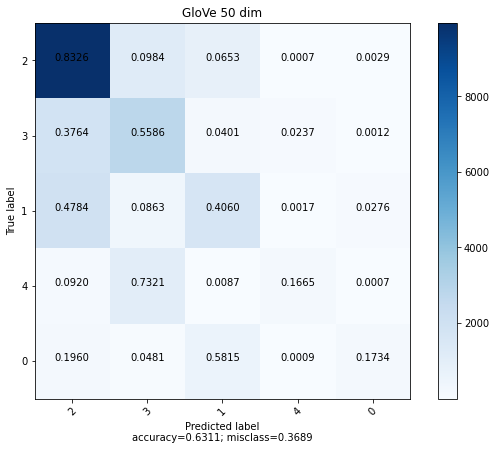
\includegraphics[scale=0.4]{../code/images/GloVe50.png}
    \caption{Confusion matrix for GloVe embedding with 50 dimensions}
    \label{fig:g50}
\end{figure}
\begin{figure}[ht]
    \centering
    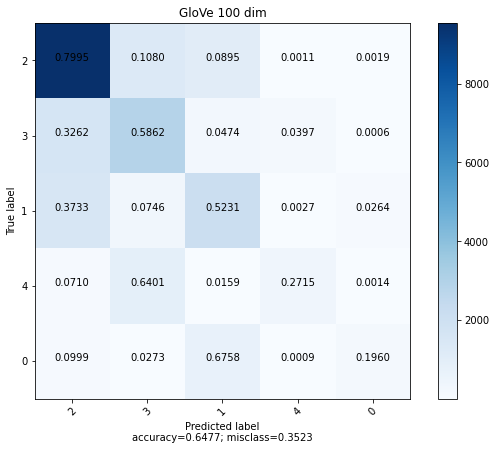
\includegraphics[scale=0.4]{../code/images/GloVe100.png}
    \caption{Confusion matrix for GloVe embedding with 100 dimensions}
    \label{fig:g100}
\end{figure}
\begin{figure}[ht]
    \centering
    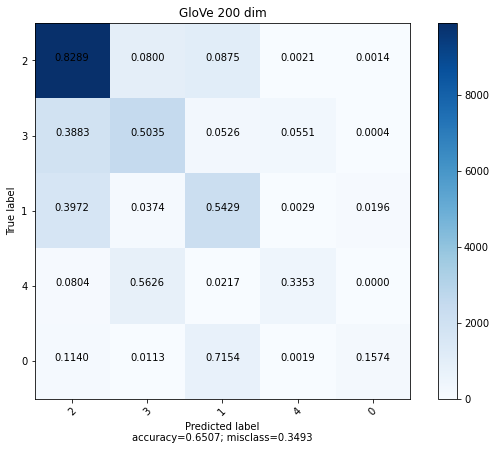
\includegraphics[scale=0.4]{../code/images/GloVe200.png}
    \caption{Confusion matrix for GloVe embedding with 200 dimensions}
    \label{fig:g200}
\end{figure}
\begin{figure}[ht]
    \centering
    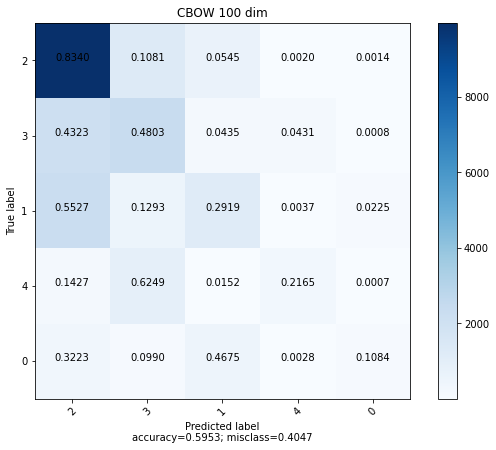
\includegraphics[scale=0.4]{../code/images/CBow100.png}
    \caption{Confusion matrix for CBOW embedding with 100 dimensions}
    \label{fig:c100}
\end{figure}
\begin{figure}[ht]
    \centering
    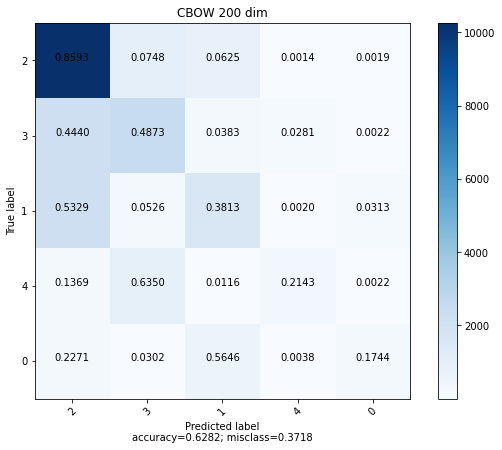
\includegraphics[scale=0.4]{../code/images/CBow200.png}
    \caption{Confusion matrix for CBOW embedding with 200 dimensions}
    \label{fig:c200}
\end{figure}
\begin{figure}[ht]
    \centering
    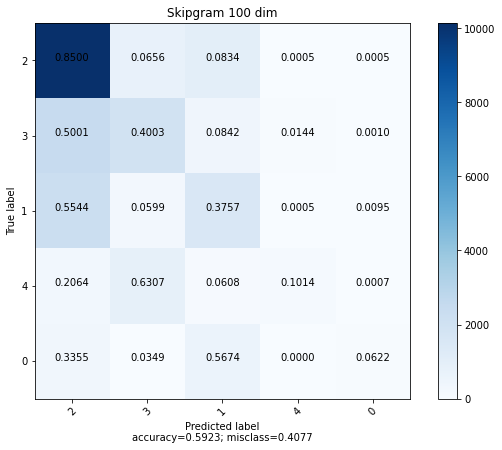
\includegraphics[scale=0.4]{../code/images/SkipGram100.png}
    \caption{Confusion matrix for Skipgram embedding with 100 dimensions}
    \label{fig:s100}
\end{figure}
\begin{figure}[ht]
    \centering
    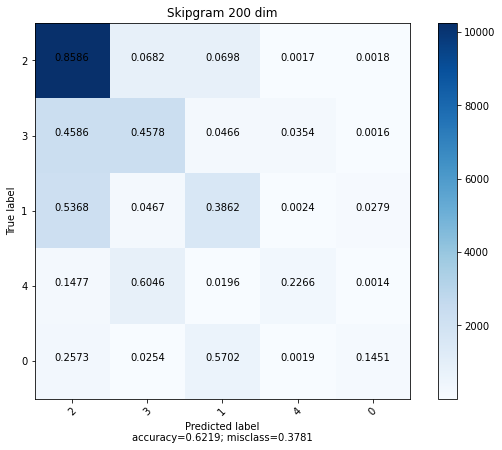
\includegraphics[scale=0.4]{../code/images/SkipGram200.png}
    \caption{Confusion matrix for Skipgram embedding with 200 dimensions}
    \label{fig:s200}
\end{figure}
After analyzing the figures, we see that the Glove embeddings produce balanced output for all classes, compared to the CBOW and Skipgram embeddings. \cref{fig:g50} to \cref{fig:s200} show plots of the confusion matrices of every LSTM model with the appropriate embedding. 
\end{document}
